UI is the graphic feature of the application mainly responsible for the displaying information and interact with the user. UI consist of login subsystem responsible for taking userid and password from user. Registration subsystem is responsible to take userid, email, password, full name from the user. Add\_Shelf subsystem is responsible for taking the shelf description from the user. Add\_Item is responsible for taking item description from user. Search subsystem is responsible for taking user input via QR code or input text. After any kind input and options chosen by the user UI\_Controller will send all user input and the option chosen by the user to Business\_Controller in Business\_Logic. UI\_Controller also accept the input messages from the Business\_Controller, stating successful completion of the chosen task by the user.

\subsection{Layer Hardware}
Being an android/iOS app, UI will use components underlying hardware for user input and to show output to the user. i.e. user uses phone screen for input and show output in same screen.

\subsection{Layer Operating System}
Android/IOS.

\subsection{Layer Software Dependencies}
We used React-Native as our frame work with the dependencies as:
\begin{rand}\\dependencies:\\ {
    "expo": "34.0.1",\\
    "expo-permissions": "6.0.0",\\
    "native-base": "2.13.7",\\
    "react": "16.8.3",\\
    "react-native": 
\end{rand}

\subsection{UI Controller}

\begin{figure}[h!]
	\centering
 	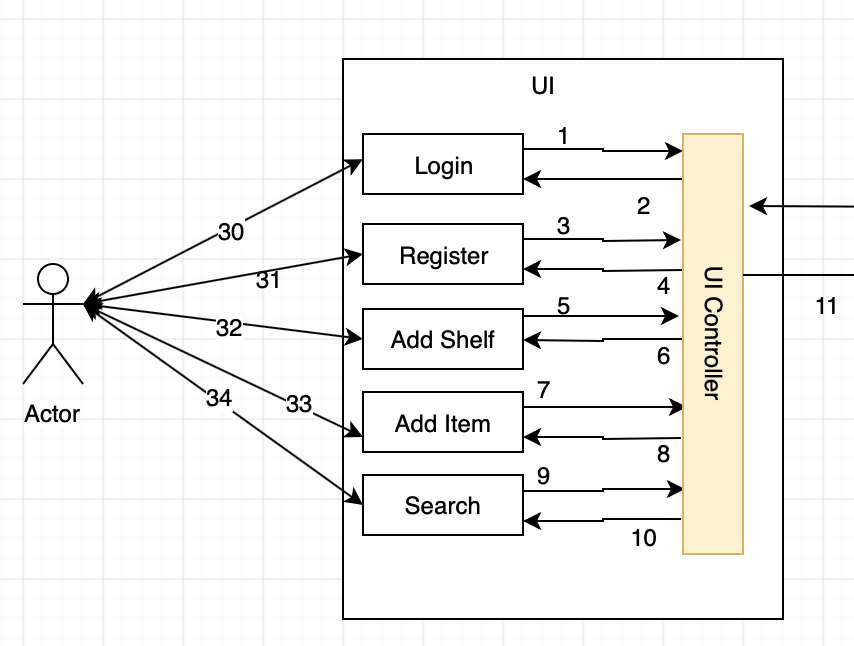
\includegraphics[width=0.60\textwidth]{images/uicontroller.png}
 \caption{Example subsystem description diagram}
\end{figure}

\subsubsection{Subsystem Hardware}
Phone Screen for both input and output.

\subsubsection{Subsystem Operating System}
Android/IOS.

\subsubsection{Subsystem Software Dependencies}
\begin{rand}dependencies:\\ {
    "expo": "34.0.1",\\
    "expo-permissions": "6.0.0",\\
    "native-base": "2.13.7",\\
    "react": "16.8.3",\\
    "react-native": 
    "react-native-datepicker": "1.7.2",\\
    "react-native-gesture-handler": "1.4.1",\\
    "react-native-search-bar": "3.4.3",\\
    "react-native-simple-radio-button": "2.7.3",\\
    "react-native-vector-icons": "6.6.0",\\
    "react-native-web": "0.11.4",\\
    "react-navigation": "4.0.0",\\
    "react-navigation-stack": "1.5.1",\\
    "reinput": "3.7.1"]\\
\end{rand}

\subsubsection{Subsystem Programming Languages}
JavaScript

\subsubsection{Subsystem Data Structures}
All types of data are transmitted as linked list or array or Union types.

\subsubsection{Subsystem Data Processing}
Our application uses sorting algorithm to sort items in the database, and authenticate using database.
\\
\\
\subsection{Login}


\begin{figure}[h!]
	\centering
 	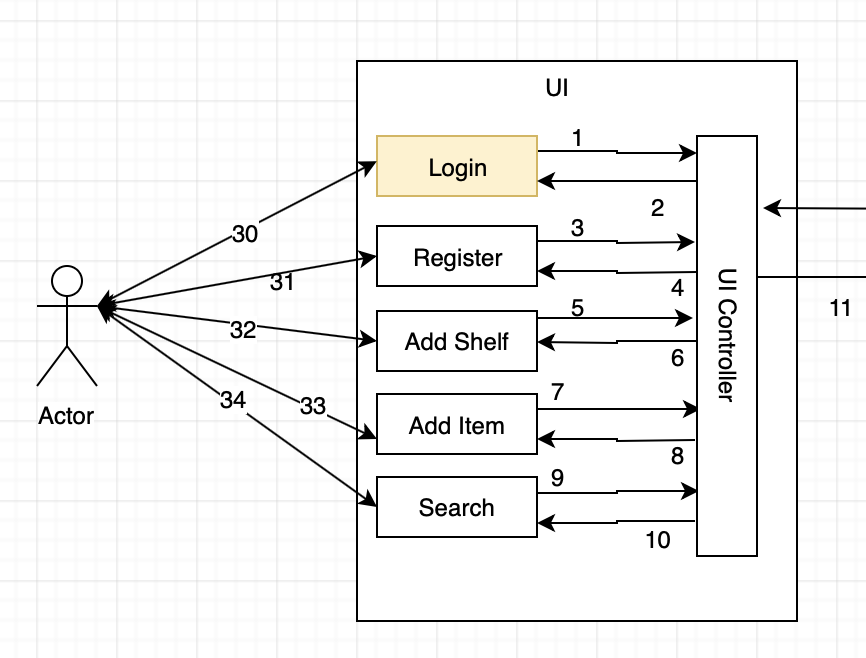
\includegraphics[width=0.60\textwidth]{images/login}
 \caption{Login description diagram}
\end{figure}

\subsubsection{Subsystem Hardware}
Phone Screen for both input and output.

\subsubsection{Subsystem Operating System}
Android/IOS.

\subsubsection{Subsystem Software Dependencies}
\begin{rand}dependencies:\\ {
    "expo": "34.0.1",\\
    "expo-permissions": "6.0.0",\\
    "native-base": "2.13.7",\\
    "react": "16.8.3",\\
     "firebase": "^6.6.0",\\
    "react-native": 
    "react-native-web": "0.11.4",\\
    "react-navigation": "4.0.0",\\
    "reinput": "3.7.1"]\\
\end{rand}

\subsubsection{Subsystem Programming Languages}
JavaScript

\subsubsection{Subsystem Data Structures}
All types of data are transmitted as linked list.

\subsubsection{Subsystem Data Processing}
This layer uses user input for authenticating for valid user.
\\
\\

\subsection{Register}


\begin{figure}[h!]
	\centering
 	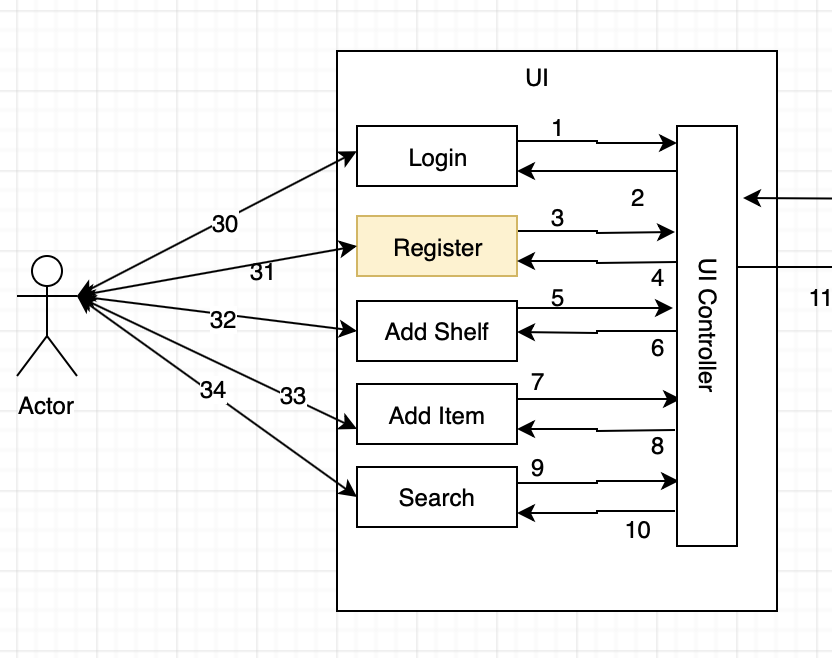
\includegraphics[width=0.60\textwidth]{images/register}
 \caption{Register description diagram}
\end{figure}

\subsubsection{Subsystem Hardware}
Phone Screen for both input and output.

\subsubsection{Subsystem Operating System}
Android/IOS.

\subsubsection{Subsystem Software Dependencies}
\begin{rand}dependencies:\\ {
    "expo": "34.0.1",\\
    "expo-permissions": "6.0.0",\\
    "native-base": "2.13.7",\\
    "react": "16.8.3",\\
     "firebase": "^6.6.0",\\
    "react-native": 
    "react-native-web": "0.11.4",\\
    "react-navigation": "4.0.0",\\
    "reinput": "3.7.1"]\\
\end{rand}

\subsubsection{Subsystem Programming Languages}
JavaScript

\subsubsection{Subsystem Data Structures}
All types of data are transmitted as linked list.

\subsubsection{Subsystem Data Processing}
This layer uses user input for authenticating for valid user and add the new user to the database.
\\
\\

\subsection{Add Shelf}


\begin{figure}[h!]
	\centering
 	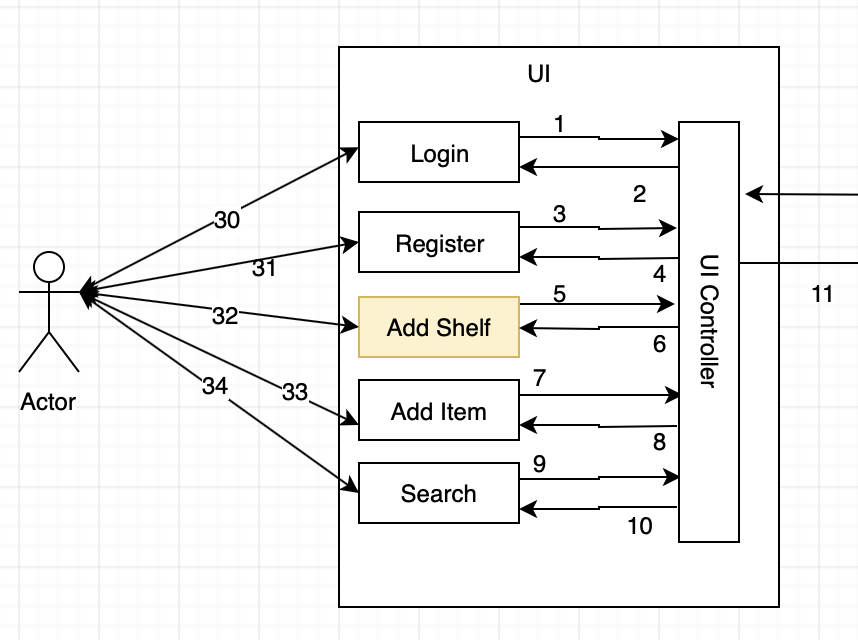
\includegraphics[width=0.60\textwidth]{images/addshelf}

 \caption{Adding Shelf description diagram}

\end{figure}

\subsubsection{Subsystem Hardware}
Phone Screen for both input and output.

\subsubsection{Subsystem Operating System}
Android/IOS.

\subsubsection{Subsystem Software Dependencies}
\begin{rand}dependencies:\\ {
    "expo": "34.0.1",\\
    "expo-permissions": "6.0.0",\\
    "native-base": "2.13.7",\\
    "react": "16.8.3",\\
     "firebase": "^6.6.0",\\
    "react-native": 
    "react-native-web": "0.11.4",\\
    "react-navigation": "4.0.0",\\
    "reinput": "3.7.1"]\\
\end{rand}

\subsubsection{Subsystem Programming Languages}
JavaScript

\subsubsection{Subsystem Data Structures}
All types of data are transmitted as linked list, array, union.

\subsubsection{Subsystem Data Processing}
This layer uses allow valid user to add new user entry to database.
\\
\\
\subsection{Add Item}
Add Item allows the user to add the items with the description of its different attributes. Attributes like name of product, brand name, manufacture date, best by date and size of product.


\begin{figure}[h!]
	\centering
 	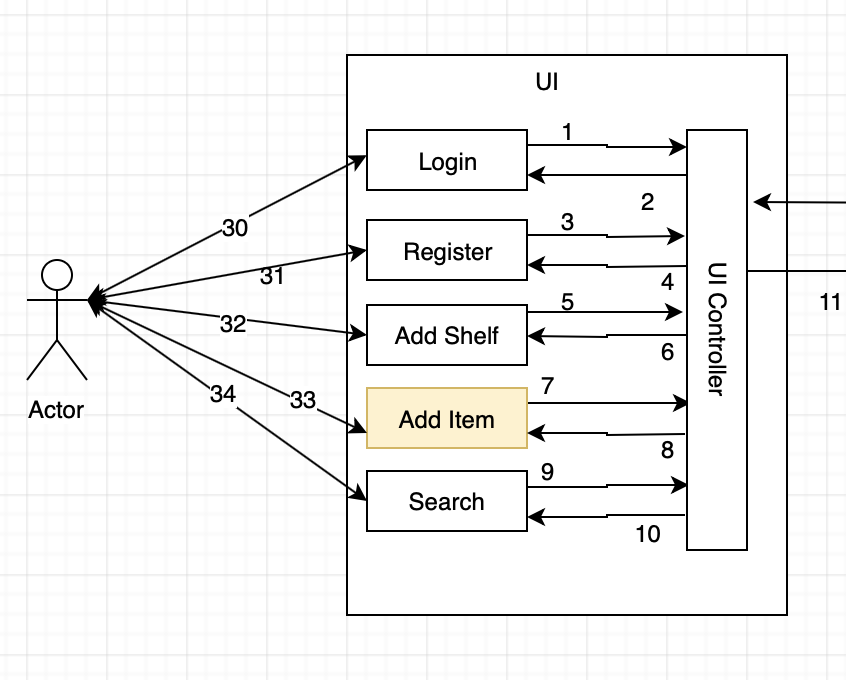
\includegraphics[width=0.60\textwidth]{images/additem}

 \caption{Adding items description diagram}

\end{figure}

\subsubsection{Subsystem Hardware}
Phone Screen for both input and output.

\subsubsection{Subsystem Operating System}
Android/IOS.

\subsubsection{Subsystem Software Dependencies}
\begin{rand}dependencies:\\ {
    "expo": "34.0.1",\\
    "expo-permissions": "6.0.0",\\
    "native-base": "2.13.7",\\
    "react": "16.8.3",\\
     "firebase": "^6.6.0",\\
    "react-native": 
    "react-native-web": "0.11.4",\\
    "react-navigation": "4.0.0",\\
    "reinput": "3.7.1"]\\
\end{rand}

\subsubsection{Subsystem Programming Languages}
JavaScript

\subsubsection{Subsystem Data Structures}
All types of data are transmitted as linked list, array, union.

\subsubsection{Subsystem Data Processing}
This layer uses allow valid user to add new user entry to database.
\\
\\
\subsection{Search}


\begin{figure}[h!]
	\centering
 	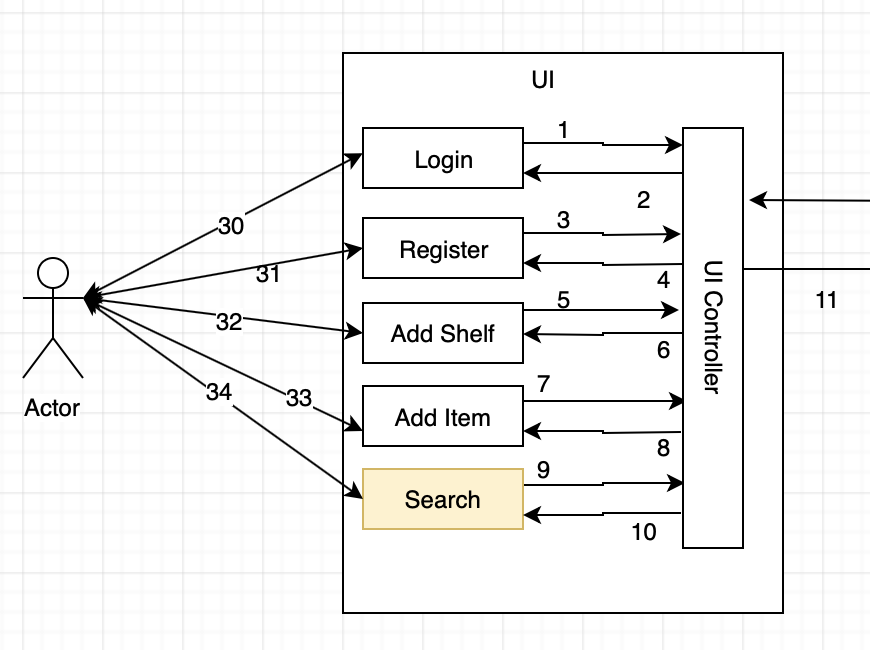
\includegraphics[width=0.60\textwidth]{images/search}
 \caption{searching item description diagram}
\end{figure}

\subsubsection{Subsystem Hardware}
Phone Screen for both input and output.

\subsubsection{Subsystem Operating System}
Android/IOS.

\subsubsection{Subsystem Software Dependencies}
\begin{rand}dependencies:\\ {
    "expo": "34.0.1",\\
    "expo-permissions": "6.0.0",\\
    "native-base": "2.13.7",\\
    "react": "16.8.3",\\
     "firebase": "^6.6.0",\\
    "react-native": 
    "react-native-web": "0.11.4",\\
    "react-navigation": "4.0.0",\\
    "reinput": "3.7.1"]\\
\end{rand}

\subsubsection{Subsystem Programming Languages}
JavaScript

\subsubsection{Subsystem Data Structures}
All types of data are transmitted as linked list, array, union.

\subsubsection{Subsystem Data Processing}
This layer uses allow valid user to search item in their database.
\\
\\

